\documentclass{article}

\usepackage{amsmath,amssymb}
\usepackage{tikz}
\usepackage{pgfplots}
\usepackage{xcolor}
\usepackage[left=2.1cm,right=3.1cm,bottom=3cm,footskip=0.75cm,headsep=0.5cm]{geometry}
\usepackage{enumerate}
\usepackage{enumitem}
\usepackage{marvosym}
\usepackage{tabularx}
\usepackage{parskip}

\usepackage{listings}
\definecolor{lightlightgray}{rgb}{0.95,0.95,0.95}
\definecolor{lila}{rgb}{0.8,0,0.8}
\definecolor{mygray}{rgb}{0.5,0.5,0.5}
\definecolor{mygreen}{rgb}{0,0.8,0.26}
%\lstdefinestyle{java} {language=java}
\lstset{language=R,
	basicstyle=\ttfamily,
	keywordstyle=\color{lila},
	commentstyle=\color{lightgray},
	stringstyle=\color{mygreen}\ttfamily,
	backgroundcolor=\color{white},
	showstringspaces=false,
	numbers=left,
	numbersep=10pt,
	numberstyle=\color{mygray}\ttfamily,
	identifierstyle=\color{blue},
	xleftmargin=.1\textwidth, 
	%xrightmargin=.1\textwidth,
	escapechar=§,
	%literate={\t}{{\ }}1
	breaklines=true,
	postbreak=\mbox{\space}
}

\usepackage[utf8]{inputenc}

\renewcommand*{\arraystretch}{1.4}

\newcolumntype{L}[1]{>{\raggedright\arraybackslash}p{#1}}
\newcolumntype{R}[1]{>{\raggedleft\arraybackslash}p{#1}}
\newcolumntype{C}[1]{>{\centering\let\newline\\\arraybackslash\hspace{0pt}}m{#1}}

\newcommand{\E}{\mathbb{E}}
\DeclareMathOperator{\rk}{rk}
\DeclareMathOperator{\Var}{Var}
\DeclareMathOperator{\Cov}{Cov}

\title{\textbf{Applied Data Analysis, Übung 5}}
\author{\textsc{Henry Haustein}}
\date{}

\begin{document}
	\maketitle
	
	\section*{Vorbereitung}
	\begin{lstlisting}
install.packages("dplyr")
library(dplyr)
install.packages("readxl")
library(readxl)
data = read_excel("data.xlsx", na = "NA")

data$gender = factor(data$gender)
levels(data$gender) = c("male", "female", "diverse")
data$employment = factor(data$employment)
levels(data$employment) = c("student", "employed", "unemployed")
data$education = factor(data$education)
levels(data$education) = c("no degree", "secondary", "intermediate", "high school", "academic")
data$play_frequency = factor(data$play_frequency)
levels(data$play_frequency) = c("never", "every few months", "every few weeks", "1-2 days a week", "3-5 days a week", "daily")
data$treatment = factor(data$treatment)
levels(data$treatment) = c("control", "lootbox in task reward", "lootbox picture", "badge")
data$age = sapply(data$age, function(year) {2016-year})
data$rt6 = as.numeric(data$rt6)
data$rt7 = as.numeric(data$rt7)
data$rt8 = as.numeric(data$rt8)
data$rt9 = as.numeric(data$rt9)
data$rt10 = as.numeric(data$rt10)
data$rt11 = as.numeric(data$rt11)
data$rt12 = as.numeric(data$rt12)
data$rt13 = as.numeric(data$rt13)
data$rt14 = as.numeric(data$rt14)
	\end{lstlisting}
	
	\section*{Task 1}
	\begin{lstlisting}
aov_tc_treatment = aov(tasks_completed ~ treatment, data = data)
summary(aov_tc_treatment)

pairwise.t.test(data$tasks_completed, data$treatment, p.adjust.method = "none")
pairwise.t.test(data$tasks_completed, data$treatment, p.adjust.method = "bonferroni")
pairwise.t.test(data$tasks_completed, data$treatment, p.adjust.method = "holm")
	\end{lstlisting}
	Ergebnis von ANOVA ist
	\begin{center}
		\begin{tabular}{lrrrrr}
  \hline
 & Df & Sum Sq & Mean Sq & F value & Pr($>$F) \\ 
  \hline
treatment & 3 & 1585.61 & 528.54 & 34.24 & $<2\cdot 10^{-16}$ \\ 
  Residuals & 433 & 6683.72 & 15.44 &  &  \\ 
   \hline
\end{tabular}
	\end{center}
	Da ANOVA auf
	\begin{itemize}
		\item $H_0: \mu_1 = \dots =\mu_g$
		\item $\exists i,j: \mu_i \neq \mu_j$
	\end{itemize}
	testet, sehen wir am p-value, dass die Treatments einen unterschiedlichen Mittelwert haben. Die paarweisen t-Tests haben folgendes Ergebnis (ohne p-value-adjustment, \textcolor{blue}{Bonferroni-Korrektur}\footnote{$p^\ast = \frac{\alpha}{n}$ mit $n$ Anzahl der Tests}, \textcolor{red}{Bonferroni-Holm Korrektur}\footnote{$p^\ast = \frac{\alpha}{m+1-k}$ mit $p_1,...,p_m$ geordneten p-values und für die $k$-te These}):
	\begin{center}
		\begin{tabular}{l|L{3.5cm}|L{3.5cm}|L{3.5cm}}
			& control & lootbox in task reward & lootbox picture \\
			\hline
			lootbox in task reward & $<2\cdot 10^{-16}$, \textcolor{blue}{$<2\cdot 10^{-16}$}, \textcolor{red}{$<2\cdot 10^{-16}$} & & \\
			\hline
			lootbox picture & 0.05967, \textcolor{blue}{0.35800}, \textcolor{red}{0.05967} & $7.3\cdot 10^{-14}$, \textcolor{blue}{$4.4\cdot 10^{-13}$}, \textcolor{red}{$3.6\cdot 10^{-13}$} & \\
			\hline
			badge & $2.8\cdot 10^{-8}$, \textcolor{blue}{$1.7\cdot 10^{-7}$}, \textcolor{red}{$1.1\cdot 10^{-7}$} & $1.9\cdot 10^{-5}$, \textcolor{blue}{0.00011}, \textcolor{red}{$5.6\cdot 10^{-5}$} & 0.00013, \textcolor{blue}{0.00079}, \textcolor{red}{0.00026}
		\end{tabular}
	\end{center}
	Wir sehen, dass bei fast allen Gruppen sich die Mittelwerte unterscheiden, bis auf $\mu_{\text{lootbox pic}} = \mu_{\text{control}}$.

	\section*{Task 2}
	\begin{lstlisting}
install.packages("car")
library(car)
data %>% group_by(treatment) %>% summarise(completeTasks_var = var(tasks_completed))
leveneTest(data$tasks_completed, data$treatment)
oneway.test(tasks_completed ~ treatment, data = data, var.equal = FALSE)

qqnorm(data$tasks_completed)
qqline(data$tasks_completed)
kruskal.test(tasks_completed ~ treatment, data = data)
	\end{lstlisting}
	Die Varianzen unterscheiden sich:
	\begin{center}
		\begin{tabular}{rlr}
  \hline
 & treatment & completeTasks\_var \\ 
  \hline
1 & control & 12.43 \\ 
  2 & lootbox in task reward & 12.29 \\ 
  3 & lootbox picture & 15.56 \\ 
  4 & badge & 19.82 \\ 
   \hline
\end{tabular}
	\end{center}
	Der Levene Test testet
	\begin{itemize}
		\item $H_0: \sigma^2_1 = \dots = \sigma^2_g$
		\item $H_1: \exists i,j: \sigma^2_i \neq \sigma^2_j$
	\end{itemize}
	und hat folgendes Ergebnis
	\begin{center}
		\begin{tabular}{lrrr}
  \hline
 & Df & F value & Pr($>$F) \\ 
  \hline
group & 3 & 14.14 & $<2\cdot 10^{-16}$ \\ 
    & 433 &  &  \\ 
   \hline
\end{tabular}
	\end{center}
	Ja, die Varianzen unterscheiden sich. Der Oneway-ANOVA-Test hat einen p-value von $<2\cdot 10^{-16}$, also gibt es auch hier Unterschiede zwischen den Gruppen.
	\begin{center}
		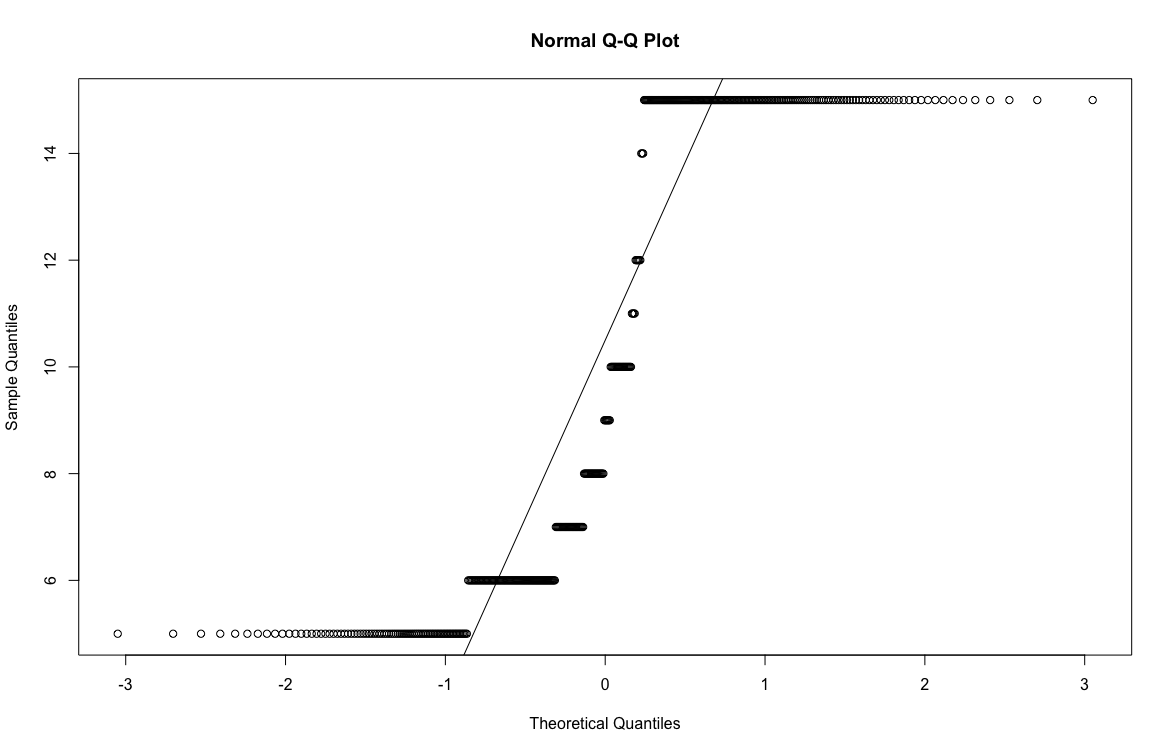
\includegraphics[scale=0.35]{qqplot.png}
	\end{center}
	Offensichtlich kann man hier auch nicht von Normalverteilung ausgehen. Der Kruskal-Wallis-Test testet, ob die Gruppen aus der gleichen Population ($H_0$) kommen. Das scheint hier nicht der Fall zu sein, der p-value ist $1.51\cdot 10^{-15}$.
\end{document}